\section{Problem 2}

This problem address multiples matching networks topologies, still using a L network, but introducing the T network and a multiple sections matching network.

\subsection{Designing the matching network}

The circuit without the matching network is a simple series association of two \texttt{Term}s component representing the source with $R_S = 500 \Omega$ and other representing the load with $Z_L = 50 + j15.9 \Omega$ at $f_o = 1 GHz$.

In a passive component representation, the load impedance can be seen as a series association of a resistance of $R_L = 50 \Omega$ with a inductance of $L_L = X_L/w_o = 2.53 \, nH$. 

Since the input impedance seen from the source must be a higher value than the actual load impedance, the L network in figure \ref{graph:2} will promote a series to parallel impedance transformation in a way that the load impedance seen from the source point-of-view is $R_{in} = R_S$.

\begin{figure}[H]
\begin{center}
\begin{tikzpicture} 
\tikzset{every pin edge/.style={scale=0.00001}    }
\begin{axis}[very thick,
                     samples = 100,
                     ytick={-0.25,2},
                     xlabel = {$t$},
                     ylabel = {$y(t)$},
                     xmin = -1,
                     xmax = 7,
                     ymin = -0.25,
                     ymax = 1.5,
                     axis x line = middle,
                     axis y line = middle,
                     ticks = none]
                     
            % waveform
            \addplot[mark=none] coordinates {(0+2,0) (1+2,1)};
            \addplot[mark=none] coordinates {(1+2,1) (3+2,0)};
            
            \addplot[mark=none] coordinates {(0+1,0) (1+1,1-0.5)};
            \addplot[mark=none] coordinates {(1+1,1-0.5) (3+1,0)};
            
            \addplot[mark=none] coordinates {(0+3,0) (1+3,1-0.5)};
            \addplot[mark=none] coordinates {(1+3,1-0.5) (3+3,0)};
            
            % labels
            \addplot[mark=none] coordinates {(1,0.2)} node[pin=270:{\scriptsize$t_d-T$}]{};
            \addplot[mark=none] coordinates {(2,0.2)} node[pin=270:{\scriptsize$t_d$}]{};
            \addplot[mark=none] coordinates {(3,0.2)} node[pin=270:{\scriptsize$t_d+T$}]{};
            \addplot[mark=none] coordinates {(0.8,1)} node[pin=180:{$A$}]{};
            \addplot[mark=none] coordinates {(0.9,0.5)} node[pin=180:{$A/2$}]{};
            
            % dashed line
            \addplot[dashed] coordinates {(0,1) (3,1)};
            \addplot[dashed] coordinates {(0,0.5) (4,0.5)};
            
            
        \end{axis}
\end{tikzpicture}
\end{center}
\caption{Forma de onda do sinal $y(t)$, como uma composição de sinais $g(t)$, com : $t_d>T$.}
\label{graph:2} 
\end{figure}

This circuit differs from the previous because it introduces a inductance in the load impedance. But this does not present any problem, since the network of figure \ref{graph:2} introduces a inductor in series with the load and its value can be found disregarding  the load inductance and after concluding the project, the load inductance can be deducted from the network inductance.

As seen in figure \ref{graph:2}(a), the impedance gain must amplify the value of the load impedance such in equation \ref{eq:6}.

\begin{equation} \label{eq:6}
    R_{in} = R_L(1+Q_s^2)
\end{equation}

The quality factor for the series association is \ref{eq:7}:

\begin{equation} \label{eq:7}
    Q_s = \sqrt{\frac{R_in}{R_{L}}-1} = 3
\end{equation}

Since the inductance of the matching network is in a series association with the load, the series quality factor is also found as the relation between the reactance with the resistance, resulting in a expression for the network inductance \ref{eq:8}.

\begin{equation} \label{eq:8}
    Q_s = \frac{L\omega_o}{R_L} \Longrightarrow L = \frac{Q_sR_L}{\omega_o} = 23.87 \, nH
\end{equation}

To calculate the network capacitance we need to transform the parallel L portion in a RLC series association, transforming L in its series equivalent with equation \ref{eq:9}.

\begin{equation} \label{eq:9}
    L_s = \frac{L}{1+Qp^{-2}} = 26.53 \, nH
\end{equation}

The capacitance can be easily found by the resonance frequency expression \ref{eq:10}.

\begin{equation} \label{eq:10}
    \omega_o = \frac{1}{\sqrt{L_sC}} \Longrightarrow C = \frac{1}{L_s \omega^2} = 0.9549 \, pF
\end{equation}

Yet the true value of L was not found, and its results from subtracting the load inductance $L_L = 2.53 \, nH$ from the result in \ref{eq:8}, so we have $L = 21.34 \, nH$.

The figure \ref{fig:smith4} illustrates the smith chart representing a match ($|S_{11}| \approx 0$) and the input impedance corresponding to the new source impedance $Z_{in} \approx 500 \Omega$ at $1 GHz$.

\begin{figure}[H] 
\centering
\includegraphics[width=7.5cm]{images/smith4.PNG}
\caption{Circuit $R_S=500 \Omega$ and $R_L=50 \Omega$ with matching network.}
\label{fig:smith4} 
\end{figure}

As a matter of comparison on future topics, we have designed a second L type matching network for a circuit with $R_S=20 \Omega$, $R_L=100 \Omega$ and $f_o = 10 GHz$ using the same methodology as before and same matching network topology (like in figure \ref{graph:1}), with quality factor $Q = 2$, inductance $L = 0.7958 \, nH$ and capacitance $C = 0.3979 \, pF$.

\subsection{Bandwidth comparison of matching network topologies}

This section will compare the previous circuit bandwidth with new impedance matching networks. Aiming an easy design for these additional networks, we will use the ADS impedance match tool \texttt{Impedance Matching}. The additional networks will obey the specifications below:

\begin{itemize}
    \item T-network with intermediate impedance $R_i = 1 k \omega$;
    \item T-network with intermediate impedance $R_i = 5 k \omega$;
    \item Low-Q three sections network;
\end{itemize}

Both the T-networks were designed using two L-network impedance match blocks in a cascade association, carefully choosing the corresponding intermediate impedance of each block to correspond the specification.

It is interesting to see that both intermediate impedances from the T-networks have higher values than input impedance. Also the input impedance is higher than the load impedance. This allow us to analyze that the impedance gain in the L-section close to the load is higher than the other section and the input impedance behaviour is to rise above the desired value and drop to the source impedance. This design pattern can be observed in the figure \ref{graph:3}. For a higher bandwidth the designer would want a minimum rise in the impedance in each section that allow a low-Q.


\begin{figure}[H]
\centering
\tikz \node [scale=0.8, inner sep=0] {
\begin{tikzpicture} 
    \draw[black, very thick] (-2,1) -- (0,1);
    \draw[black, very thick] (0,1) -- (0,3);
    \draw[black, very thick] (0,3) -- (2,3);
    \draw[black, very thick] (2,3) -- (2,-1);
    \draw[black, very thick] (2,-1) -- (4,-1);
    \node[blue] at (-2.4,1) {$R_{in}$};  
    \node[red] at (4.4,-1) {$R_{L}$}; 
    \node[black] at (1,3.4) {$R_{i}$}; 
    \node[black] at (-1.2,2) {$1+Q_2^2$}; 
    \node[black] at (3.2,1) {$1+Q_1^2$}; 
    \draw[>=latex, <->] (-0.2,1) -- (-0.2,3);
    \draw[>=latex, <->] (2.2,-1) -- (2.2,3);
    \node[black] at (0,-1.5) {(a)};
\end{tikzpicture}
};
\hspace{1cm}
\tikz \node [scale=0.8, inner sep=0] {
\begin{tikzpicture} [american]
    \draw[>=triangle 90, ->] (-2.5,0) -- (-1.5,0);
    \draw[>=triangle 90, ->] (6.5,0) -- (5.5,0);
    \draw[] (2,0.3) -- (2,0.8);
    \draw[>=triangle 90, ->] (2,0.3) -- (2.5,0.3);
    \node[black] at (2,1.2) {$R_{i}$}; 
    \node[black] at (-2.9,0) {$R_{in}$}; 
    \node[black] at (6.9,0) {$R_L$}; 
    \node[black] at (2,-4) {(b)};
    \draw (2,0) to[L, l=$L_1$, *-*] (5,0)
    (2,0) to[C, l=$C$, *-] (2,-3) node[ground]{}
    (-1,0) to[L, l=$L_2$, *-*] (2,0)
    ;
\end{tikzpicture}
};

\caption{(a) Desired effect of impedance gain(b) T matching network for a serial to parallel transformation of load impedance. Source: own.}
\label{graph:3} 
\end{figure}

The low-Q three sections network is more complex since it has two intermediate impedance and these have to be found to minimize the steps in the input impedance in each given L-network, therefore ensuring the low-Q characteristic. Once we are using the ADS tool for impedance matching, there is only the need to find the set of intermediate impedance. 

The overall low-Q three sections network is as seen in figure \ref{graph:4}. 


\begin{figure}[H]
\centering
\tikz \node [scale=0.7, inner sep=0] {
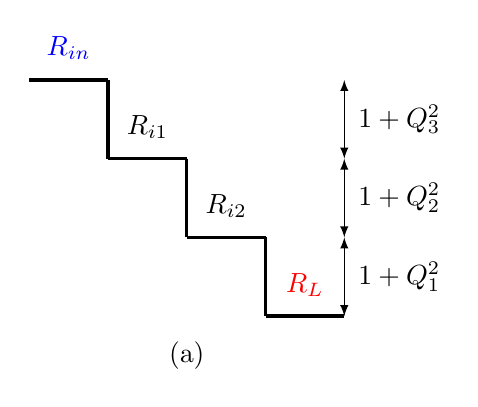
\begin{tikzpicture} 
    \draw[black, very thick] (-2,3) -- (-1,3);
    \draw[black, very thick] (-1,3) -- (-1,2);
    \draw[black, very thick] (-1,2) -- (0,2);
    \draw[black, very thick] (0,2) -- (0,1);
    \draw[black, very thick] (0,1) -- (1,1);
    \draw[black, very thick] (1,1) -- (1,0);
    \draw[black, very thick] (1,0) -- (2,0);

    \node[blue] at (-1.5,3.4) {$R_{in}$};  
    \node[red] at (1.5,0.4) {$R_{L}$}; 
    
    \node[black] at (-0.5,2.4) {$R_{i1}$};
    \node[black] at (0.5,1.4) {$R_{i2}$};
    
    \node[black] at (2.7,2.5) {$1+Q_3^2$}; 
    \node[black] at (2.7,1.5) {$1+Q_2^2$};
    \node[black] at (2.7,0.5) {$1+Q_1^2$};
    
    \draw[>=latex, <->] (2,3) -- (2,2);
    \draw[>=latex, <->] (2,2) -- (2,1);
    \draw[>=latex, <->] (2,1) -- (2,0);
    \node[black] at (0,-0.5) {(a)};
\end{tikzpicture}
};
\hspace{1cm}
\tikz \node [scale=0.7, inner sep=0] {
\begin{tikzpicture} [american]
    \draw[>=triangle 90, ->] (-5.5,0) -- (-4.5,0);
    \draw[>=triangle 90, ->] (6.5,0) -- (5.5,0);
    \draw[] (2,0.3) -- (2,0.8);
    \draw[>=triangle 90, ->] (-1,0.3) -- (-0.5,0.3);
    \draw[] (-1,0.3) -- (-1,0.8);
    \draw[>=triangle 90, ->] (2,0.3) -- (2.5,0.3);
    \node[black] at (2,1.2) {$R_{i1}$}; 
    \node[black] at (-1,1.2) {$R_{i2}$}; 
    \node[black] at (-5.9,0) {$R_{in}$}; 
    \node[black] at (6.9,0) {$R_L$}; 
    \node[black] at (0.5,-4) {(b)};
    \draw (2,0) to[L, l=$L_1$, *-*] (5,0)
    (2,0) to[C, l=$C_1$, *-] (2,-3) node[ground]{}
    (-1,0) to[L, l=$L_2$, *-*] (2,0)
    (-1,0) to[C, l=$C_2$, *-] (-1,-3) node[ground]{}
    (-4,0) to[L, l=$L_3$, *-*] (-1,0)
    (-4,0) to[C, l=$C_3$, *-] (-4,-3) node[ground]{}
    ;
\end{tikzpicture}
};

\caption{(a) Desired effect of impedance gain(b) Low-Q three sections network. Source: own.}
\label{graph:4} 
\end{figure}

The total gain correspond to the relation between input and output impedance:

\begin{equation} \label{lQ:1}
    m_{tot} = \frac{R_{in}}{R_L} = \frac{500}{50} = 10
\end{equation}

Once we are using a three section matching network ($n=3$), the impedance gain in each section will be equal in between them and equal to the cube root of the total gain:

\begin{equation} \label{lQ:2}
    m = m_1 = m_2 = m_3 = \sqrt[n]{m_{tot}} = \sqrt[3]{10} = 2.1544
\end{equation}

So after each step the corresponding intermediate impedance and, therefore the input impedance will be:

\begin{equation} \label{lQ:3}
    \begin{aligned}
        R_{i1} = m R_L = 107.72 \, \Omega \\
        R_{i2} = m R_{i1} = 232.07 \, \Omega \\
        R_{in} = m R_{i2} = 500 \, \Omega 
    \end{aligned}
\end{equation}

The same reasoning can be applied for a matching network of p-th order.

Simulating all four networks together we obtain the graph in the figure \ref{fig:bw3}. The first simulation regarding $S(2,1)$ in a solid red line refers to the first matching network designed in the begin of this problem and it is a L-network. Looking to the two T-networks with different intermediate impedances, one regarding $S(4,3)$ with a dot-dash black line and $R_i = 1 k\Omega$ and the another network regarding $S(6,5)$ with a dashed blue line and $R_i = 5 k\Omega$. We can see that the T-network insert a degree of freedom to manipulate the quality factor (therefore the bandwidth) without changing the impedance gain. This degree of freedom is does not exist in the L-network, so this topology do not allow a change in the bandwidth without changing the impedance gain.

When we rose the intermediate impedance from $1k\Omega$ to $5k\Omega$ in the T-network the bandwidth of the transmission coefficient became narrow, this is because we rose the quality factor turning the matching network more selective to the desired frequency.

\begin{figure}[H] 
\centering
\includegraphics[width=8cm]{images/BW3.PNG}
\caption{Circuit $R_S=500 \Omega$ and $R_L=50 \Omega$ with four different matching networks.}
\label{fig:bw3} 
\end{figure}

In the plot for the low-Q three L-sections network, regarding $S(6,5)$ with dotted cyan line, we can see a different effect from the one obtained before rising the intermediate impedances. In this case the bandwidth rose, since we are ensuring a low-Q.

The effect of a large or narrow bandwidth depends on application specifics and how to achieve this bandwidth is a matter of design to choose the ideal matching network topology to ensure a high quality product and lowest cost.
